\subsection{Problem}

\renewcommand{\theequation}{\theenumi}
\begin{enumerate}[label=\thesection.\arabic*.,ref=\thesection.\theenumi]
\numberwithin{equation}{enumi}
\item Find the area of the region in the first quadrant enclosed by the x-axis, the line $\myvec{1&-1}\vec{x}=0$ and the circle $\norm{\vec{x}}=1$.
The following python code computes the required area represented in Fig.\ref{fig:qseventeen}.
	\begin{lstlisting}
	./codes/circle/q17.py
	\end{lstlisting}
	
\solution The required area is given by
\begin{align} 
ar\brak{OACB} = ar\brak{OAB} + ar\brak{ACB}\\
ar\brak{OACB} = \int\limits_{0}^{0.707} x dx + \int\limits_{0.707}^{1} \sqrt{1-x^2}dx
\end{align}
which on computing, we obtain the required area as 0.3924
\begin{figure}[!ht]
	\centering
	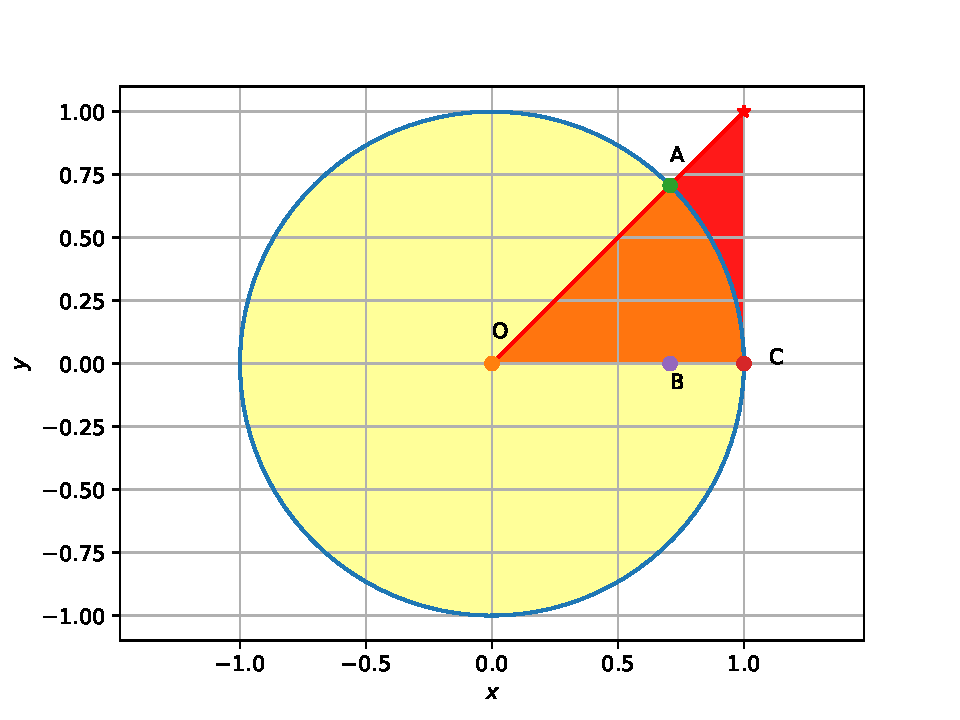
\includegraphics[width=\columnwidth]{./figs/circle/q17.pdf}
	\caption{Figure of Q.4.1.5}
	\label{fig:qseventeen}	
	\end{figure}
	
\end{enumerate}
